%MIT OpenCourseWare: https://ocw.mit.edu
%RES.18-011 Algebra I Student Notes, Fall 2021
%License: Creative Commons BY-NC-SA 
%For information about citing these materials or our Terms of Use, visit: https://ocw.mit.edu/terms.

\section{Linear Groups}

Today we'll study \textbf{linear groups} -- subgroups of matrices which satisfy conditions about preserving properties that come from linear algebra. We've seen a couple of these already. We can start off with the group $GL_n(\mathbb{R})$ of all invertible $n \times n$ matrices, and consider a few subgroups that we've seen:
\begin{center}
    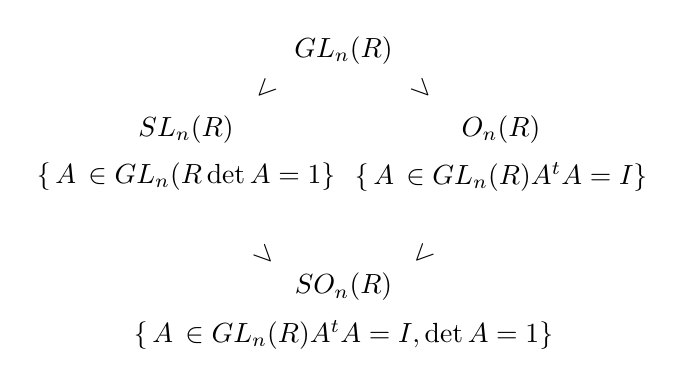
\begin{tikzpicture}[scale=2]
        \node (GLR) at (0, 1.5) {$GL_n(\mathbb{R})$};
        \node [label=below:{$\left\{\begin{matrix} A \in GL_n(\mathbb{R} \\ \det A = 1 \end{matrix}\right\}$}] (SLR) at (-1, 1) {$SL_n(\mathbb{R})$};
        \node [label=below:{$\left\{\begin{matrix} A \in GL_n(\mathbb{R}) \\  A^tA = I \end{matrix}\right\}$}] (OR) at (1, 1) {$O_n(\mathbb{R})$};
        \node [label=below:{$\left\{\begin{matrix}A \in GL_n(\mathbb{R}) \\ A^tA = I, \det A = 1 \end{matrix}\right\}$}] (SOR) at (0, 0) {$SO_n(\mathbb{R})$};
        \node [rotate=45] at (-0.5, 1.25) {$<$};
        \node [rotate=135] at (0.5, 1.25) {$<$};
        \node [rotate=135] at (-0.5, 0.2) {$<$};
        \node [rotate=45] at (0.5, 0.2) {$<$};
    \end{tikzpicture}
\end{center}
These subgroups all preserve some interesting property:
\begin{itemize}
    \item $SL_n(\RR) \leq GL_n(\RR)$ consists of the matrices with determinant 1, which preserve volume.
    \item $O_n(\RR) \leq GL_n(\RR)$ consists of the orthogonal matrices, which preserve the dot product (or equivalently, which preserve length) -- meaning that $\langle Av, Aw\rangle = \langle v, w\rangle$ for any two vectors $v$, $w$ (where the pairing denotes the dot product). 
    \item $SO_n(\RR)$ is the intersection of $SL_n(\RR)$ and $O_n(\RR)$. 
\end{itemize}

We can do the same thing for matrices with complex values:
\begin{center}
    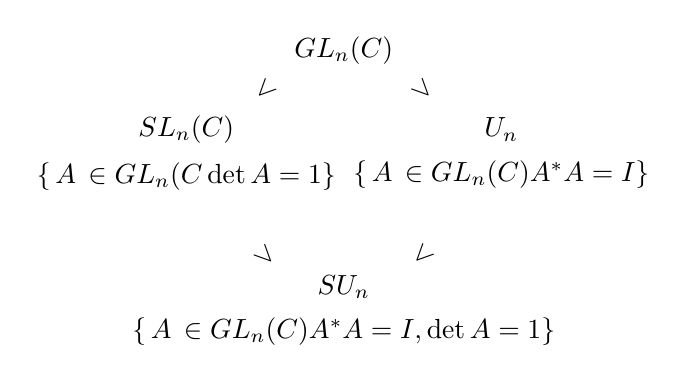
\begin{tikzpicture}[scale=2]
        \node (GLR) at (0, 1.5) {$GL_n(\mathbb{C})$};
        \node [label=below:{$\left\{\begin{matrix} A \in GL_n(\mathbb{C} \\ \det A = 1 \end{matrix}\right\}$}] (SLC) at (-1, 1) {$SL_n(\mathbb{C})$};
        \node [label=below:{$\left\{\begin{matrix} A \in GL_n(\mathbb{C}) \\  A^*A = I \end{matrix}\right\}$}] (U) at (1, 1) {$U_n$};
        \node [label=below:{$\left\{\begin{matrix}A \in GL_n(\mathbb{C}) \\ A^*A = I, \det A = 1 \end{matrix}\right\}$}] (SU) at (0, 0) {$SU_n$};
        \node [rotate=45] at (-0.5, 1.25) {$<$};
        \node [rotate=135] at (0.5, 1.25) {$<$};
        \node [rotate=135] at (-0.5, 0.2) {$<$};
        \node [rotate=45] at (0.5, 0.2) {$<$};
    \end{tikzpicture}
\end{center}
These subgroups still preserve some linear algebraic property:
\begin{itemize}
    \item $SL_n(\CC) \leq GL_n(\CC)$ is still the group of matrices with determinant $1$, the same as in the real case. 
    \item $U_n(\CC) \leq GL_n(\CC)$ is the group of unitary matrices, which preserve the standard Hermitian form -- so $\langle Av, Aw\rangle = \langle v, w\rangle$ where the pairing is now the standard Hermitian form (instead of the dot product, as in $O_n(\mathbb{R})$ for the real numbers).  
    \item $SU_n(\CC)$ is the intersection of $SL_n(\CC)$ and $U_n(\CC)$, the group of unitary matrices with determinant $1$.
\end{itemize}
We could also look at groups of matrices that preserve other bilinear forms, not just the dot product. For example, we could define the bilinear form $I_{p,q}$ corresponding to the matrix $\begin{bmatrix} I_p & \\ & -I_q \end{bmatrix}$. 
Then we could study the matrices preserving this bilinear form, meaning the set $\{A \mid A^t I_{p,q} A = I_{p, q}\}$, which is an interesting subgroup of $GL_n(\mathbb{R})$. 

\subsection{Geometry of groups}

All these matrices are over $\RR$ or $\CC$. What's special about the real or complex numbers, as opposed to something like a finite field, is that we have a notion of \emph{distance}. More explicitly, we have $GL_n(\mathbb{R}) \subset \mathbb{R}^{n^2}$ (where we just write down the coordinates), so $GL_n(\mathbb{R})$ inherits a \textbf{metric} -- we can discuss whether two elements are close together or far apart. The same works for $GL_n(\mathbb{C}) \subset \mathbb{R}^{2n^2}$ (since we can think of a complex number as a pair of real numbers). 

The actual metric itself won't be that important; what will be important is the idea of a \textbf{topology} on this set -- we have a sense of two elements being close together or far apart, which we didn't have when we studied finite or discrete groups. With finite or discrete groups, we can't really talk about a sequence of elements getting closer and closer to another, but with these groups we can. The group structure and topology interact with each other in extremely interesting ways -- these groups are called \textbf{Lie groups}, and the study of such groups ends up being a really rich vein of mathematics.

Today we'll see a flavor of how we can take a group and look at it not just as a collection of things, but also as having some sort of geometry. 

There are some questions we can ask: groups come with multiplication law, $G \times G \rto G$. It turns out that for all the matrix groups considered above, the multiplication law is continuous (if you perturb two elements a bit, this only perturbs their product a bit as well). The inverse map $g \mapsto g^{-1}$ is also continuous. Similarly, we can look at \emph{continuous} homomorphisms. 

We've seen a few simpler examples of groups with a shape (not necessarily matrix groups) -- for example, $(\RR, +)$ is just the real line:
\begin{center}
    \begin{asy}
    unitsize(3cm);
    draw((0, 0)--(2, 0), Arrows);
    \end{asy}
\end{center}

\begin{example}
How can we draw the group of $2$-dimensional rotations \[SO_2 = \{\rho_\theta \mid 0 \leq \theta < 2\pi\}?\] 
\end{example}

\begin{proof}
    On a homework problem, we showed that $SO_2 \cong \mathbb{R}/2\pi \mathbb{Z}$. So we can draw $SO_2$ as a circle, where the angle represents the angle of rotation:
    \begin{center}
        \begin{asy}
            import geometry;
            unitsize(2cm);
            draw(circle((0, 0), 1));
            draw((1, 0)--(0, 0)--dir(40));
            markangle("$\theta$", radius=10, (1, 0), (0, 0), dir(40));
        \end{asy}
    \end{center}
    We have a homomorphism $\mathbb{R} \to SO_2$ where we send $\theta \mapsto \rho_\theta$. Geometrically, this corresponds to wrapping the line around the circle infinitely many times. 
\end{proof}

Similarly, we can consider $O_2$ -- we saw that $SO_2$ has two cosets, itself and the set of reflections. So we can think of $O_2$ as two circles (with one circle representing each). 

\begin{note}
We haven't really defined terms like continuous, metric, or topology. But we won't be that formal here; instead, the main goal is to try to visualize our groups in terms of these pictures. 
\end{note}

\subsection{Geometry of \texorpdfstring{$SU_2$}{SU2}}

All the groups whose geometry we've looked at so far are one-dimensional. Now we'll look at a higher-dimensional group, the \textbf{special unitary group} \[SU_2 = \{ A \in GL_2 (\CC) \mid \det A = 1, A^* = A^{-1} \}.\] We'll try to figure out what the points in this set look like, as a geometric shape. 

\subsubsection{Quaternions}

First we'll analyze what matrices are in $SU_2$. Consider a matrix $A = \begin{bmatrix} \alpha & \beta \\ \gamma & \delta \end{bmatrix}$. Then we have \[A^{-1} = \frac{1}{\det A} \begin{bmatrix} \delta & -\beta \\ -\gamma & \alpha \end{bmatrix} = \begin{bmatrix} \delta & -\beta \\ -\gamma & \alpha \end{bmatrix}\] (since the determinant is $1$), and \[A^* = \begin{bmatrix} \overline{\alpha} & \overline{\gamma} \\ \overline{\beta} & \overline{\gamma} \end{bmatrix}.\] These must be equal, so we must have $\delta = \overline{\alpha} $ and $\beta = - \overline{\gamma}$. 
Thus we must have \[A = \begin{bmatrix}\alpha & \beta \\ -\overline{\beta} & \overline{\alpha} \end{bmatrix}.\] Finally, the condition that $\det A = 1$ means that $|\alpha|^2 + |\beta|^2 = 1$. 

We can write any matrix $A$ as a linear combination of other matrices, by splitting up the real and imaginary parts of $\alpha$ and $\beta$. Suppose $\alpha = x_0 + i x_1$ and $\beta = x_2 + i x_3$ where $x_0, x_1, x_2, x_3 \in \RR$. Then we have
\[ A = x_0 \begin{bmatrix} 1 & 0 \\ 0 & 1\end{bmatrix} + x_1 \begin{bmatrix} i & 0 \\ 0 & -i \end{bmatrix} + x_2 \begin{bmatrix} 0 & 1 \\ -1 & 0 \end{bmatrix} + x_3 \begin{bmatrix} 0 & i \\ i & 0 \end{bmatrix} .\] 

We'll introduce some notation for these matrices. The first is just the other identity; meanwhile we define
\[ \mathbf{i} = \begin{bmatrix} i & 0 \\ 0 & -i \end{bmatrix}, \, \mathbf{j} = \begin{bmatrix}0 & 1 \\ -1 & 0 \end{bmatrix}, \, \mathbf{k} = \begin{bmatrix} 0 & i \\ i & 0 \end{bmatrix} . \]


We will also define a four-dimensional real vector space consisting of all matrices of the above form (which are linear combinations of $I$, $\mathbf{i}$, $\mathbf{j}$, and $\mathbf{k}$:
\[\mathbb{H} = \RR^4 = \{x_0 I + x_1 \mathbf{i} +x_2 \mathbf{j} + x_3 \mathbf{k} \mid x_0, x_1, x_2, x_3 \in \RR\} \subset \operatorname{Mat}_{2\times 2} (\CC).\] 
This space is closed under multiplication, since we can use the relations $\mathbf{i}^2 = \mathbf{j} = \mathbf{k}^2 = -I$, $\mathbf{i} \mathbf{j} = \mathbf{k}$, $\mathbf{j} \mathbf{i} = - \mathbf{k}$, and so on. So if we multiply any two elements of $\mathbb{H}$, we get another element of $\mathbb{H}$. 

The set $\mathbb{H}$ is called the set of \textbf{quaternions}. They're like a four-dimensional version of the complex numbers (instead of adding one square root of $-1$, we now have three). But unlike the complex numbers, multiplication isn't commutative -- so it's kind of like the field of complex numbers, but it's not a field because of the lack of commutativity. (We can still divide by nonzero elements, but we have to be careful about the order.)

But the main thing we'll use here is that it's a four-dimensional real vector space -- we've figured out how to write elements in terms of coordinates. Then $SU_2 \subset \mathbb{H}$ are exactly the quaternions such that $x_0^2 + x_1^2 + x_2^2 + x_3^2 = 1$ (since this is equivalent to the determinant condition). So $SU_2$ sits inside $\mathbb{R}^4$, and consists of all vectors with length $1$ -- this means its shape is a $3$-dimensional sphere $S^3$. 

\begin{question}
    Why is it called a 3-dimensional sphere if there are four dimensions?
\end{question}

\begin{ans}
    There's four dimensions, but we're imposing an additional condition. A sphere only consists of the boundary, not the interior (a sphere with its interior is called a \emph{ball}). So although it lives in four dimensions, it's a three-dimensional surface (because we have one constraint). Similarly, a normal sphere in $\RR^3$ is called a $2$-sphere, since its surface is two-dimensional. 
\end{ans}

\subsubsection{Geometry of the Sphere}

The $3$-sphere is very hard to picture, so let's start by drawing the 2-sphere \[S^2 = \{(x_0, x_1, x_2) :  x_0^2 + x_1^2 +x_2^2 = 0 \} \subset \RR^3.\] 

As coordinates, $S^2$ is the set of solutions to $x_0^2 + x_1^2 + x_2^2 = 1$. There are many ways of representing its coordinates, but one commonly used one is spherical coordinates, which we can think of in terms of latitude and longitude. 

The latitude lines come from taking a horizontal slice of the sphere -- formally, $\operatorname{Lat}_c = \{x_0 = c\} \cap S^2$. 

\begin{center}
        \begin{asy}
            unitsize(2.5cm);
            draw(circle((0, 0), 1));
            real latc(real a, real b) {
                return sqrt((1 - a^2)*(a^2 - b^2)/a^2);
            }
            path lat2(real a, real b) {
                return shift((0, latc(a, b)))*scale(a, b)*arc((0, 0), 1, 0, 180);
            }
            path lat1(real a, real b) {
                return shift((0, latc(a, b)))*scale(a, b)*arc((0, 0), 1, 180, 360);
            }
            draw(lat1(1, 0.2), gray);
            draw(lat2(1, 0.2), gray+dashed);
            real aq = 0.8;
            real bq = aq/5;
            draw(lat1(aq, bq), heavycyan);
            draw(lat2(aq, bq), heavycyan+dashed);
            draw(rotate(180)*lat2(aq, bq), heavycyan);
            draw(rotate(180)*lat1(aq, bq), heavycyan+dashed);
        \end{asy}
    \end{center}
The latitude lines start off as a point at the north pole $\operatorname{Lat}_1$, and then as we go downwards, they get bigger and bigger until the equator $\mathbb{E} = \operatorname{Lat}_0$, and then get smaller again until the south pole. 

Meanwhile, in the other direction, we have longitude lines, which are circles of radius $1$ that intersect the north and south pole. 
\begin{center}
        \begin{asy}
            unitsize(2.5cm);
            draw(circle((0, 0), 1));
            real latc(real a, real b) {
                return sqrt((1 - a^2)*(a^2 - b^2)/a^2);
            }
            path lat2(real a, real b) {
                return shift((0, latc(a, b)))*scale(a, b)*arc((0, 0), 1, 0, 180);
            }
            path lat1(real a, real b) {
                return shift((0, latc(a, b)))*scale(a, b)*arc((0, 0), 1, 180, 360);
            }
            draw(lat1(1, 0.2), gray);
            draw(lat2(1, 0.2), gray+dashed);
            real aq = 0.8;
            real bq = aq/5;
            draw(lat1(aq, bq), heavycyan);
            draw(lat2(aq, bq), heavycyan+dashed);
            draw(rotate(180)*lat2(aq, bq), heavycyan);
            draw(rotate(180)*lat1(aq, bq), heavycyan+dashed);
            real vr = 0.4;
            draw(rotate(90)*lat1(1, 0.4), deepgreen);
            draw(rotate(90)*lat2(1, 0.4), deepgreen+dashed);
        \end{asy}
    \end{center}
So the latitude and longitude lines give us a way of representing our location on the $2$-sphere. We can do the same for the $3$-sphere: we now have \[S^3 = \{x_0^2 + x_1^2 + x_2^2 + x_3^2 = 1\}.\] We can define latitudes in the exact same way, with  $\operatorname{Lat}_c = \{x_0 = c\} \cap S^3$. This is now the set of points with $x_0 = c$ and $x_1^2 + x_2^2 + x_3^2 = 1 - c^2$, so now our latitudes are actually $2$-spheres. So we're still taking horizontal slices (with $-1 \leq c \leq 1$), but now the latitudes are $2$-spheres of different sizes. We still have just a single point at the north and south pole, and the largest latitude is still the equator $\operatorname{Lat}_0 = \mathbb{E}$. 

We'll define the longitudes precisely a bit later. These will still be circles of radius $1$ passing through both the north and south poles $(\pm 1, 0, 0, 0)$. Just like in the $2$-sphere, every point lies on a unique latitude line, and every point except the north and south pole lies on a unique longitude line; and each pair of latitude and longitude lines intersects at exactly two points. 

We've seen now that $SU_2$ as a set is a $3$-sphere in $\mathbb{R}^4$ (using this choice of coordinates), and the $3$-sphere can be thought of geometrically as having latitudes and longitudes. It turns out we can use this geometric understanding of the $3$-sphere to understand the group structure of $SU_2$. 

\subsubsection{Latitudes}

\begin{theorem}\label{conj latitudes}
    The conjugacy classes of $SU_2$ are precisely the latitudes $\text{Lat}_c$ for $-1 \leq c \leq 1$. 
\end{theorem}

So slicing the $3$-sphere horizontally into latitudes is the same as taking the group and decomposing it into conjugacy classes. 

In particular, most of these latitudes are $2$-spheres, and are infinite -- except the north pole and the south pole, which only have one element. A point has conjugacy class of size $1$ exactly when it's in the center, so this implies that $\operatorname{Lat}_{\pm 1} = \pm I = Z(SU_2)$. We can also see this is true directly, by checking which matrices commute with every other matrix in the group; but this gives a geometric interpretation. 

\begin{proof}[Proof of Theorem \ref{conj latitudes}]
Recall that when we chose coordinates, we wrote elements of $SU_2$ as \[A = x_0\begin{bmatrix} 1 & 0 \\ 0 & 1 \end{bmatrix} + x_1\begin{bmatrix} 1 & 0 \\ 0 & -i \end{bmatrix} + x_2 \begin{bmatrix} 0 & 1 \\ -1 & 0 \end{bmatrix} + x_3\begin{bmatrix} 0 & i \\ i & 0 \end{bmatrix}.\] The main point is that the first matrix $I$ has trace $2$, while the other matrices $\mathbf{i}$, $\mathbf{j}$, and $\mathbf{k}$ all have trace $0$. So then $\trace(A) = 2x_0$. 

So taking horizontal slices has some meaning in terms of the matrices itself -- it corresponds to taking slices of $SU_2$ with constant trace. 

We can use this idea to prove the theorem. Fix $A \in SU_2$ with coordinates $(x_0, x_1, x_2, x_3)$, so we want to show that $\operatorname{Conj}(A) = \operatorname{Lat}_{x_0}$. But the latitude is exactly the set $\{A' \in SU_2 \mid \trace(A') = \trace(A)\}$. 

This immediately solves one direction -- suppose $A' \in \operatorname{Conj}(A)$, so $A' = P^{-1}AP$ for some $P$. We've seen that trace is one of the coefficients of the characteristic polynomial, so it doesn't change under conjugation. So we must have $\trace(A') = \trace(A)$, which means $\operatorname{Conj}(A) \subseteq \operatorname{Lat}_{x_0}$. 

For the other direction, we want to show that if $\trace(A') = \trace{A}$, then $A' = P^{-1}AP$ for some $P \in SU_2$. To see this, consider the polynomial $t^2 - \trace(A) t + 1$. This is the characteristic polynomial of both $A$ and $A'$ (since they both have determinant $1$). Let its roots be $\lambda$ and $\overline{\lambda}$, so $\lambda$ and $\overline{\lambda}$ are the eigenvalues of $A$ and $A'$. 

Now by the Spectral Theorem, there exists a unitary matrix $Q$ such that \[Q^{-1}AQ = \begin{bmatrix} \lambda & 0 \\ 0 & \lambda \end{bmatrix} = D,\] and a unitary matrix $Q'$ such that $(Q')^{-1}A'Q' = D$ as well. 

So $A$ and $A'$ are conjugate to the same matrix, which means they're conjugate to each other -- we have \[(Q'Q^{-1})A(Q'Q^{-1})^{-1} = A'.\] Now we're almost done, but we've overlooked one detail: the Spectral Theorem shows that $A$ and $A'$ are conjugate to each other in $U_2$, but we need to check that we can do this conjugation using matrices of determinant $1$. 

But we can actually arrange for $Q$ and $Q'$ to have determinant $1$ -- suppose we have $Q \in U_2$ with $Q^{-1}AQ = D$, and let $\det Q = \delta$. Since $Q$ is unitary, we have $Q^*Q = I$, so $\overline{\delta} \cdot \delta = 1$. So then $|\delta| = 1$. Then we can set \[\tilde{Q} = Q\begin{bmatrix} \delta^{-1/2} & 0 \\ 0 & \delta^{-1/2}\end{bmatrix}.\] The matrix on the right is unitary as well (because $|\delta| = 1$), and $\det \tilde{Q} = \delta \cdot \delta^{-1} = 1$, so then $\tilde{Q} \in SU_2$. We can check that $\tilde{Q}^{-1}A\tilde{Q} = D$ as well.

So any two matrices in the same latitude are conjugate. 
\end{proof}

\begin{note}
The main idea of this proof was the Spectral Theorem, which we used to see that if two matrices in $SU_2$ have the same trace, then they're conjugate in $U_2$. Then by a bit of messing around, we could also arrange for them to be conjugate in $SU_2$. 
\end{note}

The upshot of today is that the $3$-sphere is the union of its latitudes \[ S^3 = \bigcup_{c=-1}^1 \text{Lat}_c, \] 
and this decomposition corresponds to the group theoretic decomposition \[SU_2 = \bigcup \text{conj classes}\] (where we can identify $S^3$ and $SU_2$, and the conjugacy classes are identified with the latitudes). 

When we worked with finite groups, we had the \textbf{class equation} $|G| = \sum_{i = 1}^k |C_i|$ (where the $C_i$ are the conjugacy classes). In this setting, this doesn't make much sense, since the size of the group (and the conjugacy classes) is infinite. 

But since $S^3$ is a geometric object, we can actually consider the \emph{volume} of $SU_2$ (which is the volume of $S^3$). We can't sum over the conjugacy classes because there aren't finitely many of them, but instead we can integrate; and then instead of counting the elements in each slice, we take their $2$-dimensional volume (or area) instead. So we get the equation \[\operatorname{vol}(SU_2) = \int_{c = -1}^1 \operatorname{vol}(\operatorname{Conj}_c) \, dc.\] This is very vague, but it's possible to formalize it, and it gives an identity which is a version of the usual class equation. This ends up being a really useful idea when studying these groups further -- the idea that we can take geometric quantities and integrate them, by first integrating over conjugacy classes. 

\newpage